%\documentclass[A4,12pt]{article}
\documentclass[letterpaper,12pt]{article}
\usepackage{epsfig}
\usepackage{float}
\usepackage{amssymb,amsmath,latexsym}
\usepackage[labelformat=empty]{caption}
\usepackage{color}
\usepackage{CJKutf8}
%\usepackage[abs]{overpic}

\usepackage{graphicx}
\usepackage{epstopdf}

\usepackage{tikz}
\usetikzlibrary{arrows}
\usetikzlibrary{calc}
\usetikzlibrary{scopes}
\usetikzlibrary{shadows}
\usetikzlibrary{chains}
%\usetikzlibrary{shadows.blur}

\topmargin      0in 
\textheight     9.0in 
\headheight     -0.0in 
\headsep        0in
\textwidth      6.5in 
\oddsidemargin  0in 
\evensidemargin 0in
\parskip        0pt

\newcommand{\slfrac}[2]{\left.#1\middle/#2\right.}
\newcommand{\bm}    [1]{\mbox{\boldmath $#1$}}

\newtheorem{thm}           {Theorem}
\newtheorem{lemma}    [thm]{Lemma}
\newtheorem{prop}     [thm]{Proposition}
\newtheorem{property} [thm]{Property}
\newtheorem{defin}    [thm]{Definition}
\newtheorem{corollary}     {Corollary}

\begin{document}
  \noindent COM 5170 Wireless Communication System \hfill 113064501  Chun-Ting Lin \\

  \begin{center}
    {\bf \large  Homework V}
  \end{center}


  %--------------------------------------------------------------
  \begin{enumerate}
    \item[{\bf 1. }]  \textbf{Steering Vector} \hfill \\
      First we generate a large number of phase realization $\{\theta_i\}_{i=1}^{10^8}$  from uniform distribution $\mathcal{U}(-\pi, \pi)$
\begin{itemize}
    \item[(a)] Given $v = 20$ km/hr and $f_c = 2$GHz, the doppler shift for each $\theta_i$ is obtained by
    \begin{eqnarray*}
        f_{D, i} & = & f_m \cos\left(\theta_i\right) \\
                 & = & \frac{v}{\lambda_c} \cos\left(\theta_i\right) \\
                 & = & \frac{v}{v_c} f_c \cos\left(\theta_i\right) \quad \text{where} \quad v_c = 3 \cdot 10^8 \, m/s
    \end{eqnarray*}
    After calculating doppler shift for each $\theta_i$, we can plot the histogram of $\{f_{D,i}\}$ to see its pdf and cdf.
    \begin{figure}[H]
        \centering
        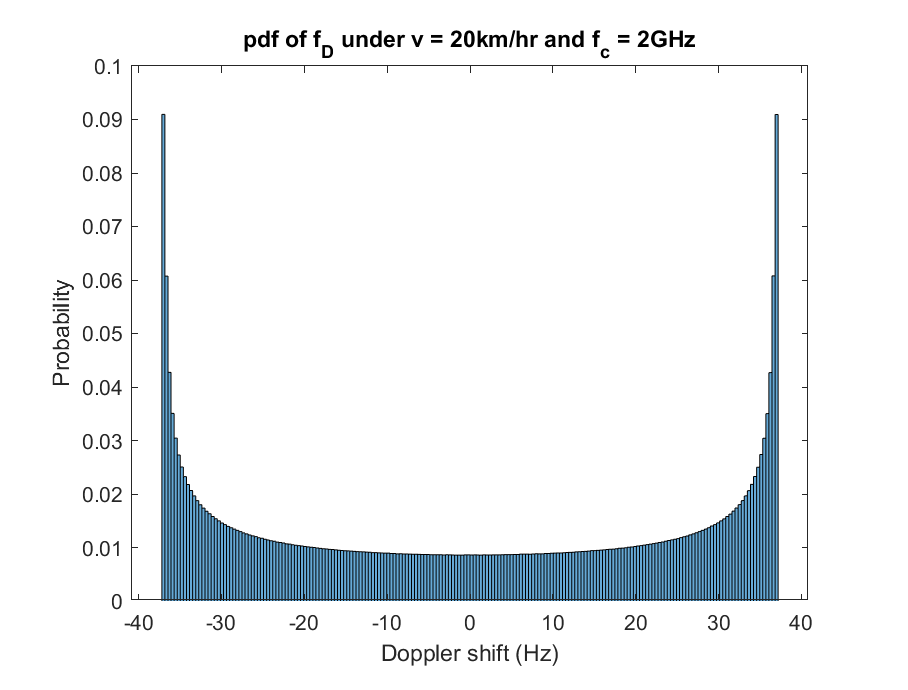
\includegraphics[scale = 0.8]{a_pdf.eps}
    \end{figure}
    \begin{figure}[H]
        \centering
        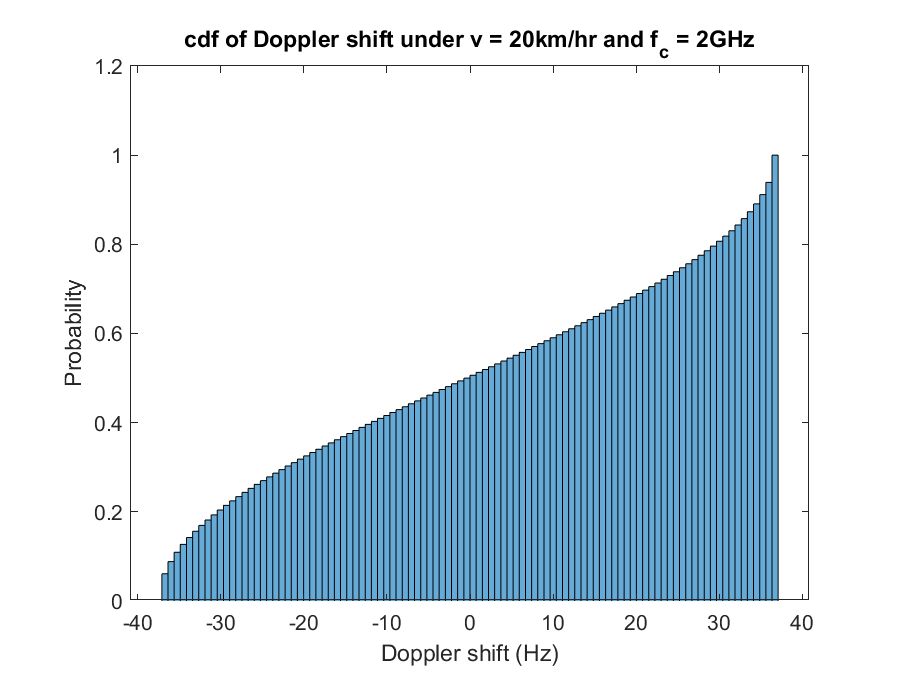
\includegraphics[scale = 0.8]{a_cdf.eps}
    \end{figure}
    \item[(b)] Totally the same as (a), just change $v$ and $f_c$.
    \begin{figure}[H]
        \centering
        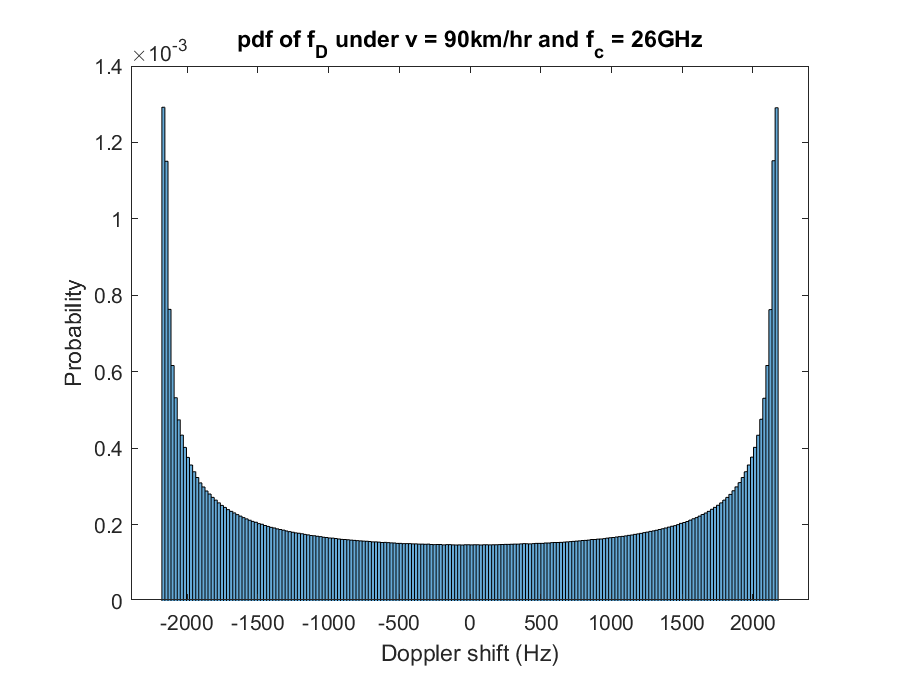
\includegraphics[scale = 0.8]{b_pdf.eps}
    \end{figure}
    \begin{figure}[H]
        \centering
        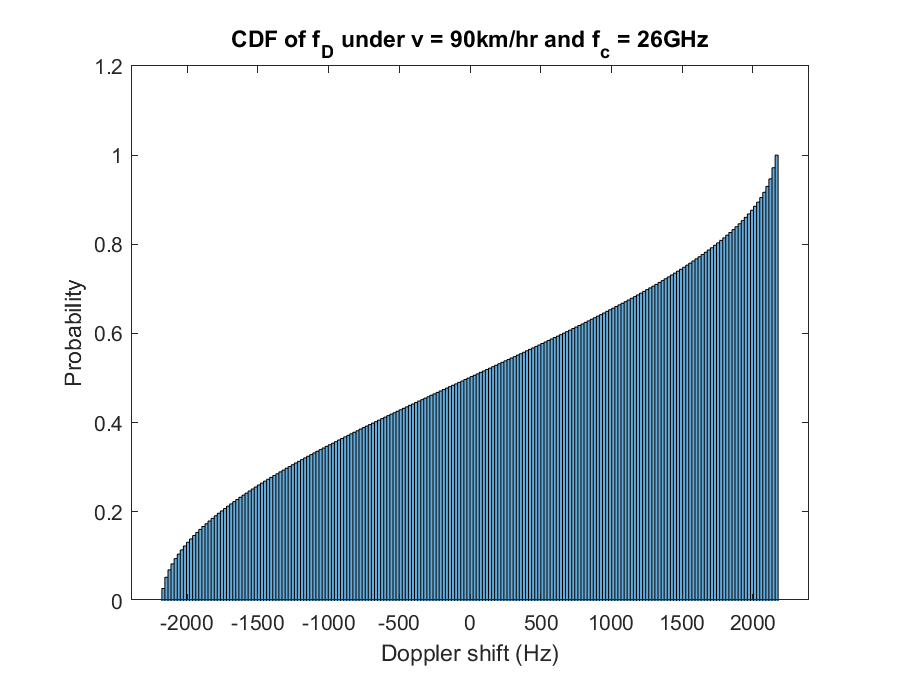
\includegraphics[scale = 0.8]{b_cdf.eps}
    \end{figure}
    \item[(c)] In this part, $v$ also becomes uniform distributed. Hence we generate same number of velocity realization $\{v_i\}_{i=1}^{10^8}$
    and use the same formula to calculate doppler shift for each pair $(v_i, \theta_i)$. 
    \begin{equation*}
        f_{D, i} = \frac{v_i}{v_c} f_c \cos\left(\theta_i\right) \quad \text{where} \quad v_c = 3 \cdot 10^8 \, m/s
    \end{equation*}
    The results are shown below
    \begin{figure}[H]
        \centering
        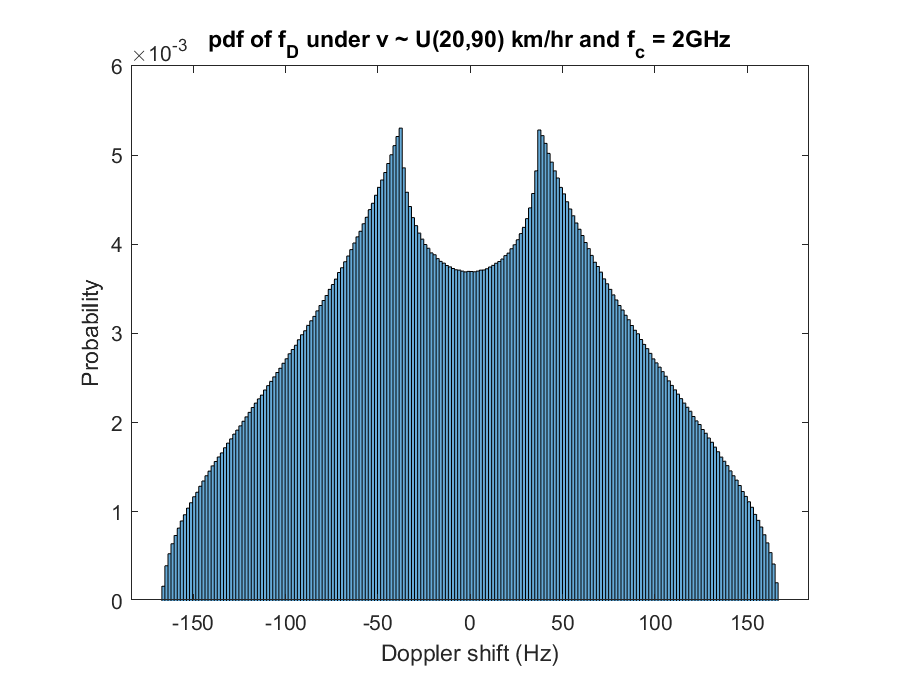
\includegraphics[scale = 0.8]{c_pdf.eps}
    \end{figure}
    \begin{figure}[H]
        \centering
        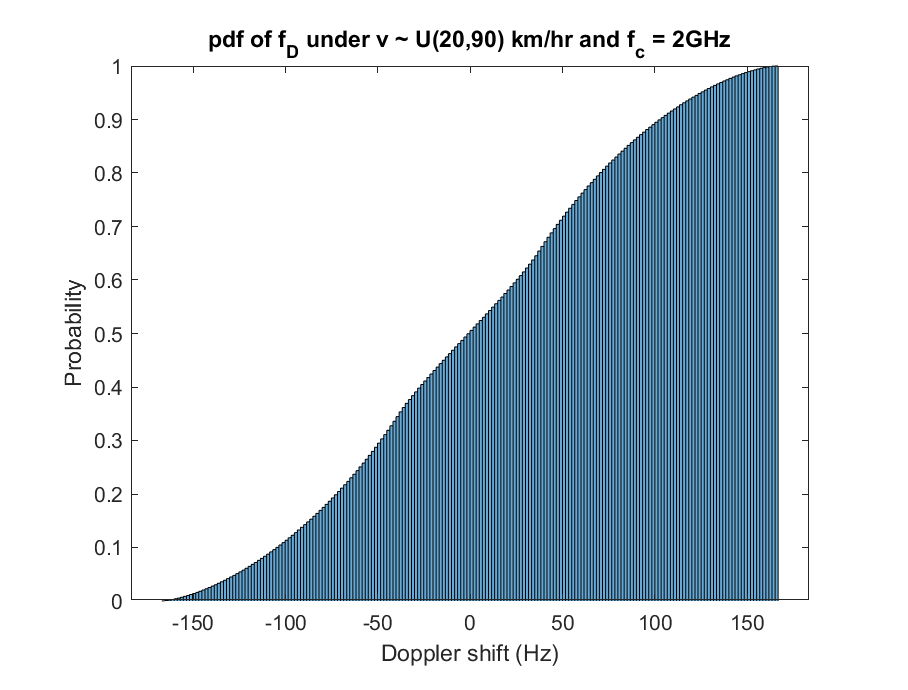
\includegraphics[scale = 0.8]{c_cdf.eps}
    \end{figure}
    \item[(d)] Now, we try to derive the pdf and cdf of $f_D$. Given 
    \begin{eqnarray}
        \theta & \sim & \mathcal{U}(-\pi, \pi) \\
        f_D    &  =   & f_m \cos \left(\theta\right)
    \end{eqnarray}
    For a certain $f_D$, the corresponding solution for (2) is 
    \begin{equation*}
        \theta_1 = \arccos \left(\frac{f_D}{f_m} \right) \quad \text{and} \quad \theta_2 = - \arccos \left(\frac{f_D}{f_m} \right).
    \end{equation*}
    Therefore, the pdf of $f_D$ is then given as
    \begin{eqnarray*}
        P(f_D) & = & \frac{1/2\pi}{\left|-f_m \sin\left(\theta_1\right)\right|} + \frac{1/2\pi}{\left|-f_m \sin\left(\theta_2\right)\right|} \\
               & = & 2 \cdot \frac{1}{2\pi} \cdot \frac{1}{\sqrt{f_m^2 - f_D^2}} \quad \left(\because \sin\left(\arccos \left(\frac{f_D}{f_m} \right)\right) = \frac{\sqrt{f_m^2 - f_D^2}}{f_m} \right)\\
               & = & \frac{1}{\pi} \cdot \frac{1}{\sqrt{f_m^2 - f_D^2}}
    \end{eqnarray*}
    The cdf of $f_D$ can further be derived
    \begin{eqnarray*}
        F(f_D) & = & \int_{-f_m}^{f_D} P(x) \, dx \\
               & = & \frac{1}{\pi \cdot f_m} \int_{-f_m}^{f_D} \frac{1}{\sqrt{1 - \left(\frac{x}{f_m}\right)^{2}}} \, dx \\
               & = & \frac{1}{\pi} \int_{-1}^{\frac{f_D}{f_m}} \frac{1}{\sqrt{1 - u^{2}}} \, du \quad \left(\text{let } u = \frac{x}{f_m}\right) \\
               & = & \frac{1}{\pi} \arcsin \left( u \right) \Bigg|_{-1}^{\frac{f_D}{f_m}} \\
               & = & \frac{1}{\pi} \arcsin\left(\frac{f_D}{f_m}\right) + \frac{1}{2}
    \end{eqnarray*}
    Plot the results with MATLAB, we get
    \begin{figure}[H]
        \centering
        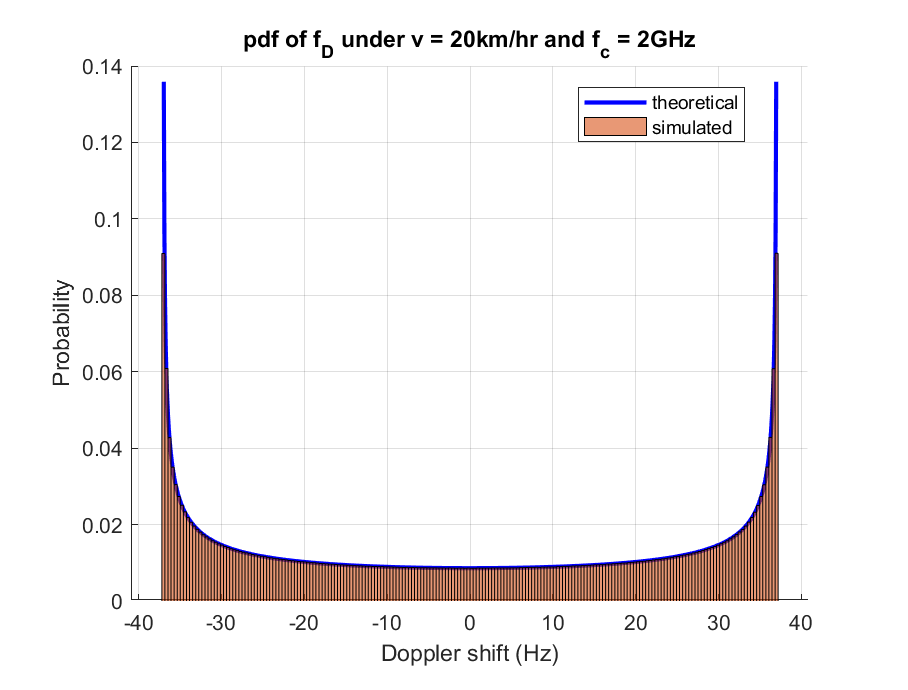
\includegraphics[scale = 0.8]{d_pdf.eps}
    \end{figure}
    \begin{figure}[H]
        \centering
        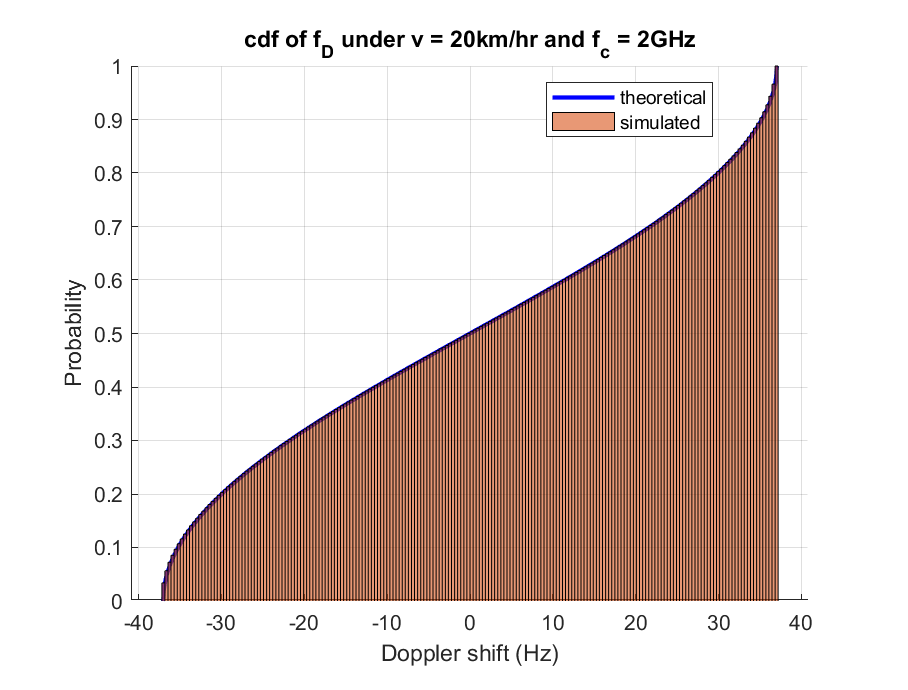
\includegraphics[scale = 0.8]{d_cdf.eps}
    \end{figure}
    The solid line is the theretical result while the histogram is the simulated result. It can be seen that 
    they look similiar.
\end{itemize}
    \item[{\bf 2. }]  \textbf{Radiation Pattern} \hfill \\
      The radiation pattern is obtained by projecting onto the target steering vector.
Suppose the incidence angle of the desired signal is $\phi_0$, the attenuation at angle 
$phi$ is
\begin{equation*}
    \text{P}\left(\phi\right) = \left|e_r^{H}(\Omega) \cdot e_r(\Omega_0)\right|
\end{equation*}
where
\begin{equation*}
    \Omega = \cos\left(\phi\right) \quad \text{and} \quad \Omega_0 = \cos\left(\phi_0\right)
\end{equation*}
The radiation patterns are shown below:
\begin{figure}[H]
    \centering
    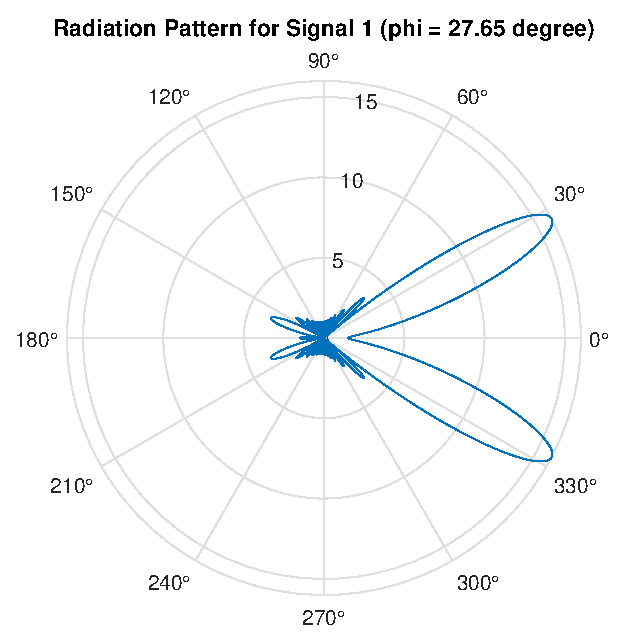
\includegraphics[scale = 0.7]{s1.eps}
\end{figure}
\begin{figure}[H]
    \centering
    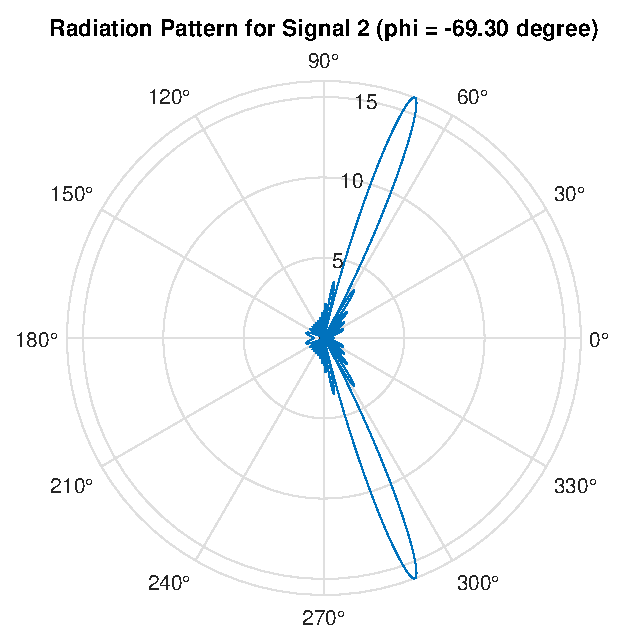
\includegraphics[scale = 0.7]{s2.eps}
\end{figure}
\begin{figure}[H]
    \centering
    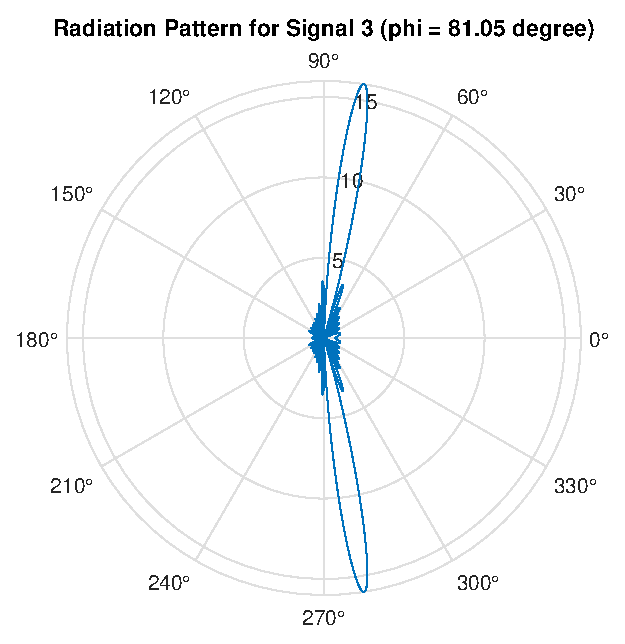
\includegraphics[scale = 0.7]{s3.eps}
\end{figure}
\begin{figure}[H]
    \centering
    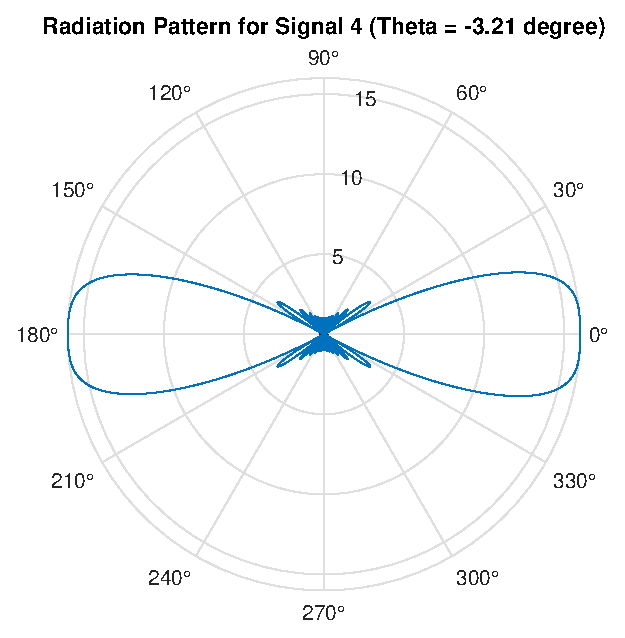
\includegraphics[scale = 0.7]{s4.eps}
\end{figure}
\begin{figure}[H]
    \centering
    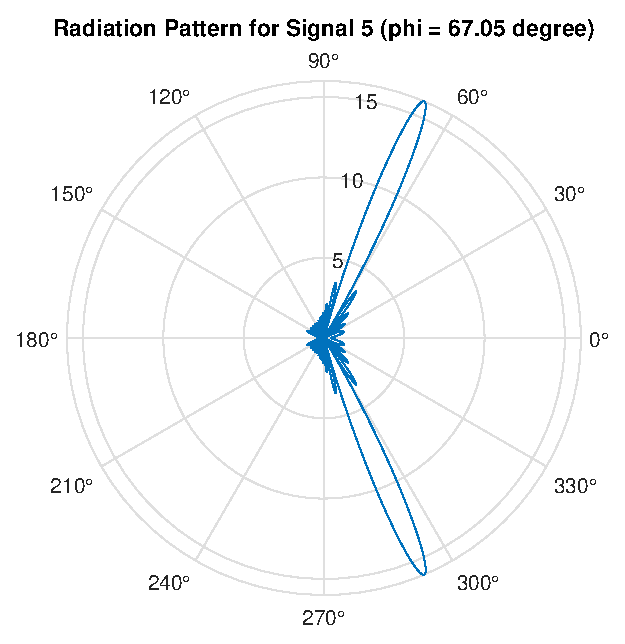
\includegraphics[scale = 0.7]{s5.eps}
\end{figure}
It can be observed that with receive beamforming, the main lobe is aligned with the incidence angle.
    \item[{\bf 3. }]  \textbf{SIR for N = 16} \hfill \\
      Similar to that in problem 2, if the incidence angle of the desired signal is $\phi_i$, then the
interference power is obtained by projecting other signals onto the steering vector of desired signal.
\begin{equation*}
    \text{P}{\scriptsize \text{interference}} = P \cdot \sum_{j \neq i} \left|e_r^{H}(\Omega_j) \cdot e_r(\Omega_i)\right|^2.
\end{equation*}
Hence, the signal-to-interference power ratio (SIR) is given by
\begin{equation*}
    \text{SIR} = \frac{\left|e_r^{H}(\Omega_i) \cdot e_r(\Omega_i)\right|^2}{\sum_{j \neq i} \left|e_r^{H}(\Omega_j) \cdot e_r(\Omega_i)\right|^2}.
\end{equation*}
The SIRs of each signal are listed in the table below:
\begin{table}[H]
    \centering
    \begin{tabular}{c|c|c|c|c|c}
             & Signal 1 & Signal 2 & Signal 3 & Signal 4 & Signal 5 \\
    \hline
    SIR (dB) & 17.7617 & 1.0028 & 13.3221 & 17.8966 & 1.2187
    \end{tabular}
\end{table}
From the table above, it can be observed that the SIR of signals 2 and 5 is close to one.
The reason is that $\phi_2$ and $\phi_5$ are close to each other. The steering vector of signal 2
also provides gain for signal 5, and vice versa. More precisely,
\begin{equation*}
    \left|e_r^{H}(\Omega_2) \cdot e_r(\Omega_2)\right|^2 \approx \left|e_r^{H}(\Omega_5) \cdot e_r(\Omega_2)\right|^2.
\end{equation*}
and
\begin{equation*}
    \left|e_r^{H}(\Omega_5) \cdot e_r(\Omega_5)\right|^2 \approx \left|e_r^{H}(\Omega_2) \cdot e_r(\Omega_5)\right|^2.
\end{equation*}
    \item[{\bf 4. }]  \textbf{SIR for N = 64} \hfill \\
      Similiar to that in (c), we may obtian the SIR for each signal under $N_r = 64$ received antenna.
The SIR of each signal is listed in the table below:
\begin{table}[H]
    \centering
    \begin{tabular}{c|c|c|c|c|c}
        & Signal 1 & Signal 2 & Signal 3 & Signal 4 & Signal 5 \\  
             \hline 
    SIR (dB) & 21.2980  & 16.7495  & 23.8789  & 21.1201  & 16.7325  
    \end{tabular}
\end{table}
Compared to that in problem 3, it can be observed that the SIR for 
each signal increases as the number of receiving antennas increases.
The reason can be seen from the radiation patterns
\begin{figure}[H]
    \centering
    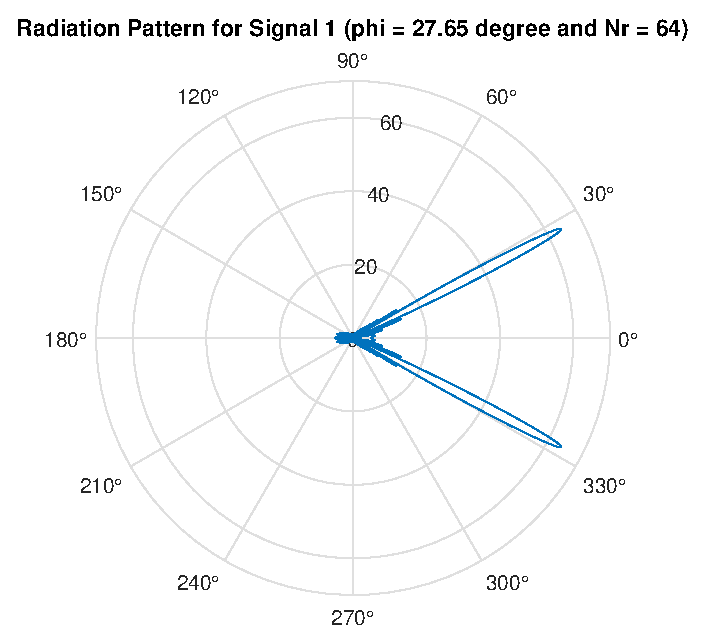
\includegraphics[scale = 0.7]{N64_1.eps}
\end{figure}
\begin{figure}[H]
    \centering
    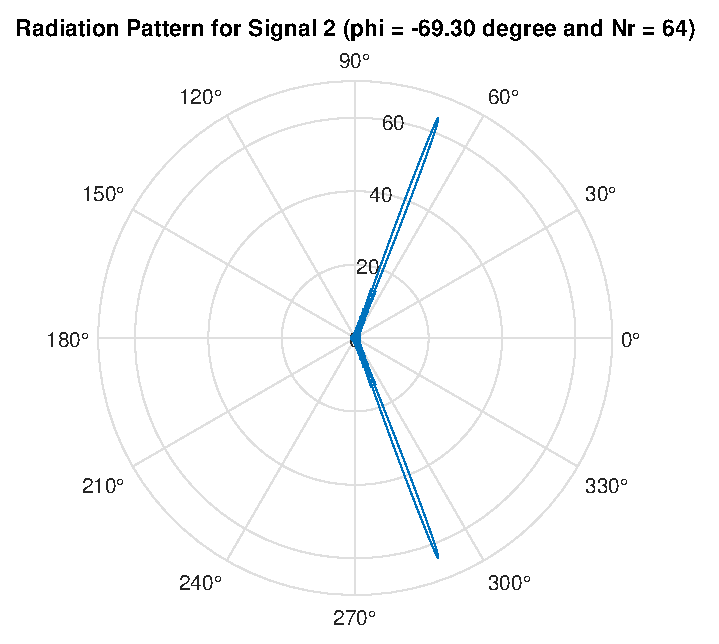
\includegraphics[scale = 0.7]{N64_2.eps}
\end{figure}
\begin{figure}[H]
    \centering
    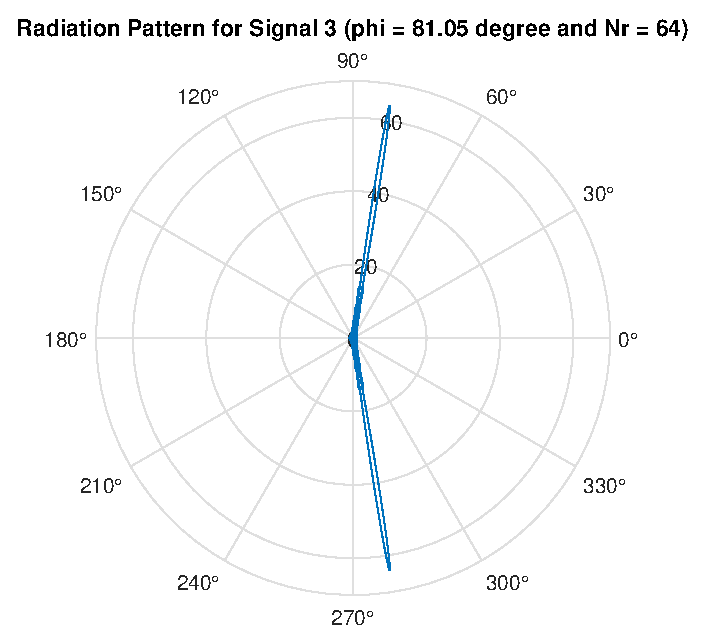
\includegraphics[scale = 0.7]{N64_3.eps}
\end{figure}
\begin{figure}[H]
    \centering
    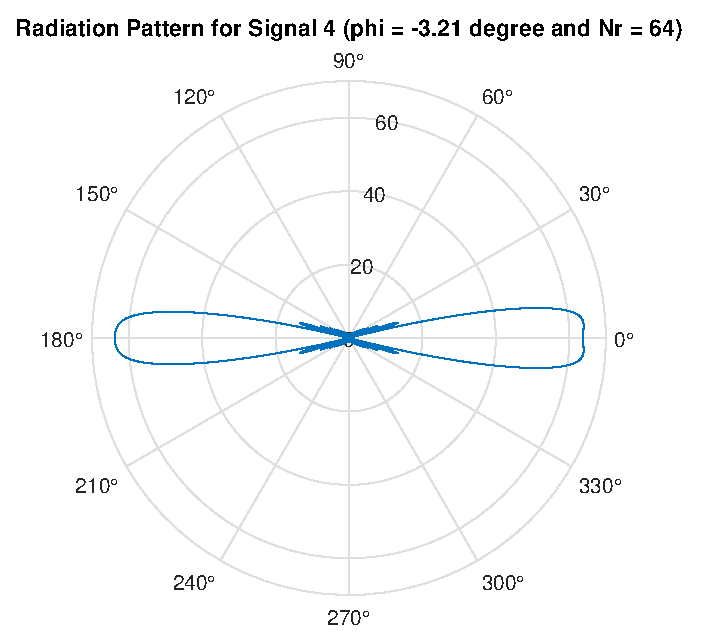
\includegraphics[scale = 0.7]{N64_4.eps}
\end{figure}
\begin{figure}[H]
    \centering
    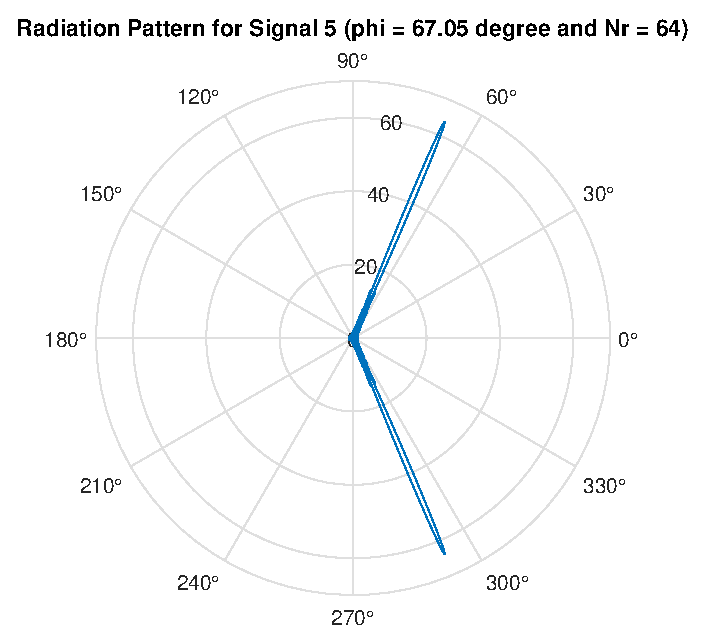
\includegraphics[scale = 0.7]{N64_5.eps}
\end{figure}
It can be seen that as $N_r$ increases, the beamwidth becomes narrower. Hence, the gain at 
angles other than the incidence angle becomes smaller, improving the angular resolvability. 
This also explains why the SIR of signals 2 and 5 is no longer 1.
  \end{enumerate}
\end{document}
